\section{Abstraction: deciding which hands share a strategy}\label{sec:abstraction}

\mkey{abstraction}Sampling makes iterations affordable; the ledgers themselves still need one row per infoset. The classical answer is \keyterm{abstraction}\mdef{abstraction}{solve a smaller merged game whose solution transfers back to the real one}: merge strategically similar situations, solve the smaller game, lift the strategy back. A decade of poker research is essentially a ratchet of better answers to ``which hands should share a row?'' --- and even though this project's endgame replaces tables with networks, the ratchet survives as the checklist for what the network's \emph{inputs} must express, and as the recipe for the dashboard's bucketed range view.

\textbf{Layer 0 --- lossless.} Some merges cost literally nothing: hands identical up to relabeling suits play identically, and Gilpin \& Sandholm~\cite{gilpin2007} proved equilibria of the merged game lift back \emph{exactly}. For Drawmaha the sweep behind this survey brute-force-verified the payoff: the 2{,}598{,}960 five-card hands collapse to exactly \textbf{134{,}459} canonical classes ($19.3\times$). \hlight{Suit-isomorphic canonicalization is free accuracy --- it should key every table, buffer, and dashboard lookup in the project regardless of any other choice.} One caveat travels with it: the $19.3\times$ shrinks as board and draw cards pin suits down --- late-street symmetry is weaker, and Waugh's perfect-indexing algorithm~\cite{waugh2013iso} is the standard way to key the canonical classes.

\textbf{Layer 1 --- a scalar per hand.} Rank every hand by \keyterm{E[HS]}\mdef{E[HS]}{expected hand strength: equity vs.\ a random opponent hand, averaged over runouts} and cut into percentile buckets. Trivial to compute, fine for a first prototype --- and blind in a specific, poker-relevant way: a made hand and a big draw can carry the \emph{same} average equity with \emph{opposite} distributions (Figure~\ref{fig:equity}), and they want opposite strategies (one wants the pot now; the other prices in cards to come).

\begin{figure}[t]
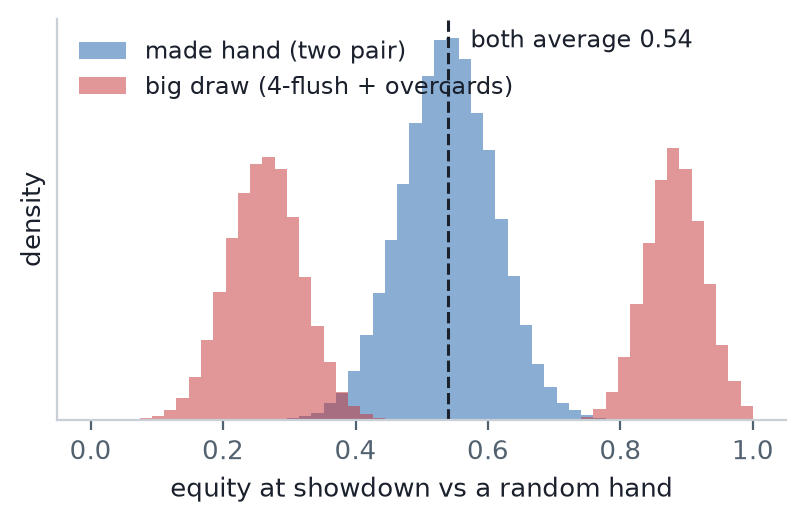
\includegraphics[width=\linewidth]{figures/equity.png}
\caption{Two hands with equal average equity and opposite equity distributions (illustrative densities): the scalar cannot see the difference; the histogram can.}
\label{fig:equity}
\end{figure}

\textbf{Layer 2 --- the distribution.} Represent each hand by its full equity \emph{histogram} over runouts and cluster the histograms with $k$-means under \keyterm{earth mover's distance}\mdef{earth mover's distance}{distance between histograms = minimum ``work'' to shovel one shape into the other} (Johanson et al.\ 2013~\cite{johanson2013}). Distribution-aware buckets beat scalar buckets on both exploitability and head-to-head play. The same study validated \keyterm{imperfect recall}\mdef{imperfect recall}{let the abstraction forget earlier-street details to spend its bucket budget on the present} --- strictly better use of a fixed budget, at the cost of voiding CFR's convergence guarantee (it works empirically; Section~\ref{sec:solving}'s perfect-recall condition is the reason the theory breaks).

\textbf{Layer 3 --- the trajectory.} Two hands can even share a final histogram but \emph{realize} it differently --- exactly the pre-draw/post-draw distinction. Potential-aware abstraction (Ganzfried \& Sandholm 2014~\cite{ganzfried2014}, the champion-agent method) represents an early-street hand by its distribution over \emph{next-street buckets}, built bottom-up, so when strength arrives matters, not just how much. \mnote{Drawmaha translation: pre-draw buckets should be distributions over post-draw buckets --- one recursive level, since there is one draw. This is literally the situation the method was invented for.}

\textbf{Actions get abstracted too.} A pot-limit tree still needs a bet-size menu (the project's v1: \{pot\} only, by design), and any \emph{deployed} strategy must interpret off-menu sizes. The standard is the \keyterm{pseudo-harmonic mapping}\mdef{action translation}{rule mapping a real-world bet onto the solver's nearest menu sizes} (Ganzfried \& Sandholm 2013~\cite{ganzfried2013at}): randomize between the neighboring menu sizes with game-theoretically derived probabilities --- naive nearest-size rounding is provably exploitable by bet sizing alone. The dashboard needs this the day it accepts a user-typed bet; the principled upgrade is re-solving off-menu spots exactly (Section~\ref{sec:search}).

Two warnings temper the whole enterprise. First, the \textbf{abstraction pathology} (Waugh et al.\ 2009~\cite{waugh2009}): \pitfall{refining an abstraction --- more buckets, finer distinctions --- can make the real-game strategy MORE exploitable; quality is non-monotonic in size}, so bucket sweeps must be validated by measured exploitability, never assumed. Second, the modern question --- \emph{doesn't deep learning make all this obsolete?} --- gets a precise answer: Deep CFR's paper claims it ``obviates the need for abstraction,'' and what it actually removes is the hand-crafted \emph{clustering}. The \emph{representation} problem survives inside the input featurization: canonical hands, card embeddings, street and pot features are abstraction moved into the network's first layer, and everything this section learned --- distribution shape matters, trajectory matters, and for Drawmaha strength is \textbf{two-dimensional} (inner equity, outer equity, scoop probability, so a scalar is even more misleading than in hold'em) --- is the checklist for those features.

\mnote{The display side reuses this machinery: an equity-histogram $k$-means into 8--20 \emph{named} buckets over the 134,459 classes is the planned range-view grouping, even though the solver itself is bucket-free.}For this project abstraction therefore lives in three places: free canonicalization everywhere; honest bucketing (layers 1--3) for the tabular mini-drawmaha stage; and feature design plus the dashboard's human-readable buckets at full scale.
